\chapter{Einleitung}
\label{cha:Einleitung}

In diesem Kapitel wird die behandelte Problemstellung und Motivation der vorliegenden Arbeit dargestellt und eine Zielsetzung definiert. Außerdem wird auf die Gliederung
dieser Arbeit eingegangen und der Inhalt der einzelnen Kapitel kurz erläutert.

\section{Motivation für den Einsatz von SCADA-Systemen}

Ein grundlegendes Problem bei der Digitalisierung von Fabriken ist, dass Cloudanwendungen, die Anlagen 
steuern und überwachen wollen, und Anlagen, wiederum deren Daten in der Cloud ablegen wollen. 
Um diesen Konflikt zu lösen, werden sogenannte SCADA-Systeme eingesetzt. SCADA ist ein Akronym und steht für Supervisory Control And 
Data Acquisition. Diese Systeme implementieren laut Automatisierungspyramide Ebene zwei und Teile von Ebene drei. 

\begin{figure}[h]
	\centering 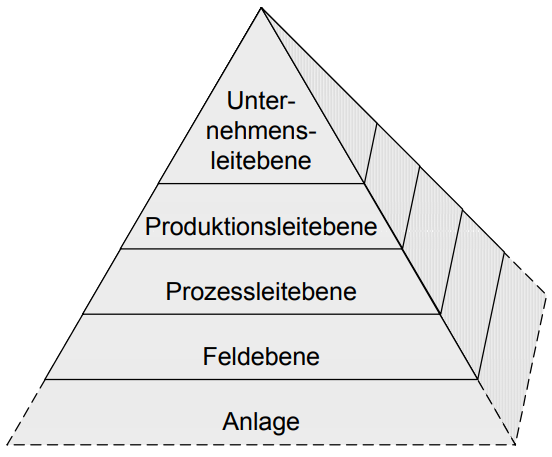
\includegraphics[width=0.58\textwidth]{aut_pyr}
	\caption{Diese Abbildung stellt die verschiedenen Ebenen der industriellen Fertigung mit Hilfe der Automatisierungspyramide dar \cite{automPyr}.
  Cloudanwendungen befinden sich in der Ebene vier, die auch \textit{Unternehmensleitebene} genannt wird.}
	\label{fig:aut_pyr}
\end{figure}

Die in Abbildung \ref{fig:aut_pyr} gezeigten Ebenen können wie folgt zusammengefasst werden \cite{Prozessleittechnik}:
\begin{itemize}
  \item Ebene vier: Die \textit{Unternehmensleitebene} umfasst Produktionsplanung und Bestellabwicklung.
  \item Ebene drei: Stellt die \textit{Produktionsleitebene} dar, in der Produktionsdaten erfasst werden. Außerdem findet hier Qualitäts- und Materialmanagement statt.
  \item Ebene zwei: In der \textit{Prozessleitebene} wird bedient, beobachtet, es werden Daten gesammelt und archiviert.
  \item Ebene eins: Steuert die Anlage über SPSen (Speicherprogrammierbaren Steuerungen), die mit dieser über Bussysteme verbunden sind. Daher wird diese Ebene auch \textit{Steuerungsebene} oder \textit{Feldebene} genannt. Weitere Teilnehmer sind unter anderem Frequenzumrichter und Industrie-PCs.
  \item Ebene null: Als \textit{Anlage} wird die zu steuernde Maschine und die dazugehörige Sensorik bezeichnet. \\
\end{itemize}

Unter SCADA versteht man das Überwachen und Steuern technischer Prozesse durch Computersysteme \cite{whatIsScada}.
Diese Systeme helfen bei der Überwachung von Anlagen und sind somit Wegbereiter, um Verfügbarkeit und Produktivität zu erhöhen. 
Am Siemensstandort in der Krausstraße in Linz befindet sich die Abteilung \textit{DF FA SO SIS}. Der
Abteilungsname beschreibt den Tätigkeitsbereich und steht als Abkürzung für Digital
Factory, Factory Automation, Solution Operation und Shopfloor IT Solutions. 
Am Standort in Linz wird unter dieser Division an der Entwicklung von Lösungen für digitalisierte Fabriken gearbeitet. 
Ein Aufgabenbereich ist hierbei der Entwurf des webbasierenden Supervisory Control And Data Acquisition (SCADA) Systems 
\textit{SiPlant} für die Automobilindustrie. Dieses Produkt kann als Erweiterung der Softwarelösung
\textit{Simatic Windows Control Center Open Architecture} (WinCC OA) der Siemens Tochtergesellschaft ETM Professional Control 
gesehen werden. WinCC OA eignet sich hierbei als Basissystem, da die Multi-Agent-Architektur ein einfaches Erweitern über eine 
C++-Programmierschnittstelle ermöglicht. Außerdem werden bereits viele Möglichkeiten zum akquirieren von Daten über proprietäre oder offene 
Feldbus Protokolle zur Verfügung gestellt. Als Beispiele können hier Profinet, MODBUS, S7Plus, OPC UA und BACNET angeführt werden \cite{WinCCOA}.
Um plattformunabhängig moderne Visualisierungen für die Überwachung von Anlagen umsetzten zu können, 
wurde für \textit{SiPlant} HTML5 als Technologie gewählt. Dies wurde mit Hilfe von eigens entwickelten WinCC OA Agenten umgesetzt.

\section{Probleme bei der Systemintegration von SCADA-Systemen}

Verschiedene Kundenstandards in den SPS-Programmen (Level 1 laut Automatisierungspyramide) und proprietäre Protokolle 
Richtung \textit{Unternehmensleitebene} führen dazu, dass bei jeder Systemintegration individuelle Probleme gelöst werden müssen.
Außerdem müssen Systemintegratorinnen und Systemintegratoren oft kundenspezifische Anwendungsfälle umsetzen. Hierbei bieten die
Bordmittel von WinCC OA oft nur eingeschränkt Möglichkeiten.

\section{Zielsetzung}

Aufgrund der Unterschiede zwischen den einzelnen Anlagen der Automatisierungsindustrie und den verschiedenen kundenspezifischen 
Projektanforderungen ist die Integration des \textit{SiPlant} Produktes oft mit vielen unvorhersehbaren und komplexen Problemen 
verbunden. Ziel dieser Arbeit ist es daher, die Google V8 Javascriptengine und das dazugehörige Debuginspector-Protokoll 
für das Produkt \textit{SiPlant} an das Basissystem WinCC Open Architecture anzubinden, um damit den Systemintegratorinnen und Systemintegratoren
ein Werkzeug für die Fehlersuche und zum Umsetzen von Kundenanforderungen mit Hilfe einer einfachen Skriptsprache zur Verfügung zu 
stellen.

\section{Gliederung dieser Arbeit}

Die vorliegende Arbeit ist in acht verschiedene Kapitel gegliedert. \autoref{cha:Einleitung} Umfasst die Motivation und Zielsetzung dieser
Arbeit.
In \autoref{cha:scadasysteme} wird definiert, was unter dem Terminus Multi-Agent-SCADA-System verstanden wird. Danach wird die Umsetzung
eines solchen anhand des Produktes \textit{Simatic Windows Control Center Open Architecture} aufgezeigt und dessen C++-Programmierschnittstelle
praktisch erklärt.
\autoref{cha:v8engine} zeigt, wie die Google V8 Javascriptengine funktioniert und wie sie von C++-Entwicklern in eigene Programme eingebettet werden
kann.
Das \autoref{cha:Anforderungen} definiert den Funktionsumfang des in dieser Arbeit entwickelten Agenten anhand von Anwendungsfällen für Systemintegratorinnen und
Systemintegratoren.
Der konzeptuelle Aufbau des Agenten, das Zusammenspiel der einzelnen Komponenten und die Umsetzung der in \autoref{cha:Anforderungen} festgelegten Anforderungen
werden in \autoref{cha:Konzept} beschrieben.
Auf Implementierung mit Hilfe der festgelegten Konzepte aus \autoref{cha:Konzept} und die Lösung aller aufkommenden Probleme wird
in \autoref{cha:Projektumsetzung} eingegangen.
In \autoref{cha:praxis} werden die durch den Einsatz des in dieser Arbeit entwickelten Agenten gesammelten Erfahrungen aufgeführt.
Das letzte \autoref{cha:Zusammenfassung} umfasst die Zusammenfassung der Erkenntnisse dieser Arbeit und ein Fazit aus den Praxiserfahrungen.
Darüber hinaus werden in einem Ausblick Vorschläge für Verbesserungen formuliert.

\section{Codebeispiele}

In dieser Arbeit werden verschiedene Konzepte und Programmierschnittstellen anhand von Codebeispielen erklärt. Diese Beispiele sind
als vollständige Projekte der CD-ROM/\\DVD beigelegt und können auf 64 Bit Systemen mit Windows 10 oder SUSE Linux Enterprise 12.5 
übersetzt werden. Dazu werden folgende Abhängigkeiten benötigt: 

\subsection{Windows 10}

\begin{itemize}
  \item Visual Studio 2019
  \item Visual Studio Toolset v140
  \item WinCC OA Version 3.16 inklusive C++-Programmierschnittstelle
  \item CMake mit mindestens Version 3.5
  \item Den SMF\_3P Ordner von der CD-ROM/DVD
\end{itemize}

\subsection{SUSE Linux Enterprise 12.5}

\begin{itemize}
  \item GCC 4.8.5
  \item WinCC OA Version 3.16 inklusive C++-Programmierschnittstelle
  \item CMake mit mindestens Version 3.5
  \item Den SMF\_3P Ordner von der CD-ROM/DVD
\end{itemize}